\documentclass[12pt,letterpaper]{article}
\usepackage{titling}
\usepackage{amsmath}
\usepackage{amssymb} 
\usepackage{graphicx} % For image
\usepackage{float} % For image H option
\usepackage{enumitem} % For enumerate
\usepackage{bm} % For bold math symbols
\usepackage{xcolor} % For color
\usepackage{subcaption} % For subfigures
\usepackage[margin=1in]{geometry}


\begin{document}
\title{\textbf{Segmentation of Vessels in Retinal Images}}
\author{Team Members: Shiyu Wang, Enhao He, Jiacheng Ma, Joe Wang}
\date{}
\setlength{\droptitle}{-2.75cm}
\maketitle
\vspace{-2cm}


\section{Introduction}
% Retinal vessel segmentation plays a critical role in the early diagnosis and treatment of various ocular diseases such as diabetic retinopathy and glaucoma. Optical characteristics such as the width, tortuosity, and overall geometry of retinal vessels can provide essential diagnostic information; however, the segmentation task itself is challenging due to vessels' complex structure, low contrast with the background, and heterogeneous illumination conditions across images. In this project, the DRIVE (Digital Retinal Images for Vessel Extraction) dataset is employed to study classical machine learning methods for vessel segmentation. In particular, we focus on K-means clustering and its optimized variants, incorporating image augmentation and gradient-based enhancements to improve segmentation accuracy.

\section{Related Work}
% Traditionally, retinal vessel segmentation was performed manually by ophthalmologists, a process that is both time-consuming and subjective. Recent developments in deep learning have led to highly accurate automated methods utilizing encoder-decoder frameworks, attention mechanisms, and transformer-based models. Despite impressive performances, these methods often require extensive computational resources and large annotated datasets. In contrast, our research revisits classical machine learning approaches—specifically K-means clustering—and proposes several optimizations to improve its effectiveness in retinal vessel segmentation.

\section{Methods}
% The overall methodology is implemented in \texttt{python} and consists of multiple stages including data loading, preprocessing, clustering, optimization, and evaluation.

\subsection{Data Loading and Preprocessing}
The DRIVE dataset is loaded by reading the retinal images, manually segmented vessel masks, and background mask data using libraries such as \texttt{tifffile}, \texttt{PIL}, and \texttt{numpy}. \\
Preprocessing part mainly focuses on the \textbf{Image Augmentation}. We enhance images using adjustments to color, brightness, and contrast (implemented in \texttt{augment\_color}) to mitigate uneven illumination and improve vessel feature clarity. \\
Besides, we also remove the background from the original image to focus on the non-background pixels by using the background mask in the dataset. 
\subsection{K-means Clustering}
K-means clustering is applied to segment the retinal images based on their RGB values. However, this approach introduces several challenges:
\begin{itemize}
    \item \textbf{Determining the Optimal Cluster Number (\texttt{n\_clusters})}: Choosing too few clusters may lead to the merging of vessel pixels with surrounding tissue, whereas an excessive number of clusters can fragment vessels, causing a discontinuous representation of the blood vessels.
    \item \textbf{Variations in Illumination and Noise}: Differences in image illumination and inherent noise can further complicate the segmentation task, making it challenging to distinguish between vessel and non-vessel regions without additional preprocessing (such as image augmentation techniques).
    \item \textbf{Limited Feature Representation}: Relying solely on RGB values can be inadequate due to the often subtle contrast between vessels and the background. This limitation might require integrating additional features (such as gradient or texture information) to capture more features of vessel morphology.
\end{itemize}



\subsubsection{Find the Best ``\texttt{n\_clusters}''}
According to the structure of normal retinal photographs, the optimal number of clusters should be \textbf{4}, including: macula (dark shadow in the center), optic disc (bright shadow on the side), blood vessels, and others. But in computer's language, more detailed exploration is still needed. \\
The approach we used involves evaluating different numbers of clusters (ranging from 2 to 10) by computing the AUC value for each image and taking the mean value. The cluster number should be at least 2, representing the vessel pixels and other tissue pixels. 
\begin{figure}[H]
    \centering
    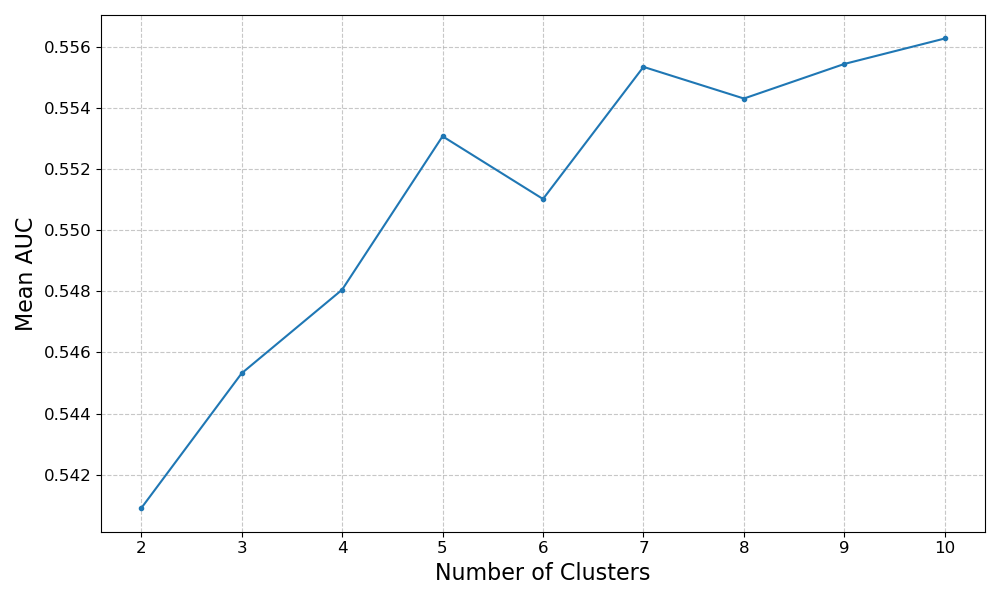
\includegraphics[scale=0.5]{Figures/1-1 Find the Best n_clusters.png}
    \caption{Mean AUC values for Different Number of Clusters.}
    \label{fig:nclusters}
\end{figure}
\noindent
As shown in Figure~\ref{fig:nclusters}, the mean AUC value \textbf{increases} with the cluster number, but the growth is gradually slowing down. \\
Then, we try to make a further decision through visualizing the segmentation results for all images with different cluster numbers, which are shown below in Figure~\ref{fig:n=2}, \ref{fig:n=6}, and \ref{fig:n=10}. 
\begin{figure}[H]
    \centering
    \includegraphics[scale=0.3]{Figures/1-2 2 Clusters.png}
    \vspace{-0.25cm}
    \caption{Segmentation Results (\texttt{n\_clusters}=2).}
    \label{fig:n=2}
\end{figure}
\vspace{-1cm}
\begin{figure}[H]
    \centering
    \includegraphics[scale=0.3]{Figures/1-2 6 Clusters.png}
    \vspace{-0.25cm}
    \caption{Segmentation Results (\texttt{n\_clusters}=6).}
    \label{fig:n=6}
\end{figure}
\vspace{-1cm}
\begin{figure}[H]
    \centering
    \includegraphics[scale=0.3]{Figures/1-2 10 Clusters.png}
    \vspace{-0.25cm}
    \caption{Segmentation Results (\texttt{n\_clusters}=10).}
    \label{fig:n=10}
\end{figure}
\noindent
There are much clearer blood vessel shapes can be observed with the increase of cluster number. However, the vessel pixels are fragmented into multiple clusters. Thus, the AUC value for a single cluster in each image is reduced and not sufficient to evaluate the segmentation performance. \\
Therefore, we decided to set \texttt{n\_clusters} = 10 as an optimal compromise with an \textbf{optimized K-means algorithm}, which can handle the merging of clusters and improve the segmentation performance. \\
To match the biological explanation at the beginning of this section, we merge the top 3 clusters with the highest AUC values to form the final vessel segmentation mask (since $10/3 \sim 4$).
\subsubsection{Optimized K-means Algorithm}
To address the challenge of correctly identifying vessel clusters, an optimized version of K-means is used. This method involves:
\begin{enumerate}
    \item Running standard K-means on non-background pixels.
    \item Evaluating each cluster by computing the AUC value between the binary prediction for that cluster and the ground truth.
    \item Merging the top-K clusters with the top 3 AUC values to form the final vessel segmentation mask.
\end{enumerate}
Figure~\ref{fig:opt} depict the three best segmentation examples using this approach, including the original image, the ground truth, the segmentation result with AUC values, and the segmentation overlay. 
\begin{figure}[H]
    \centering
    \begin{subfigure}[H]{\textwidth}
        \centering
        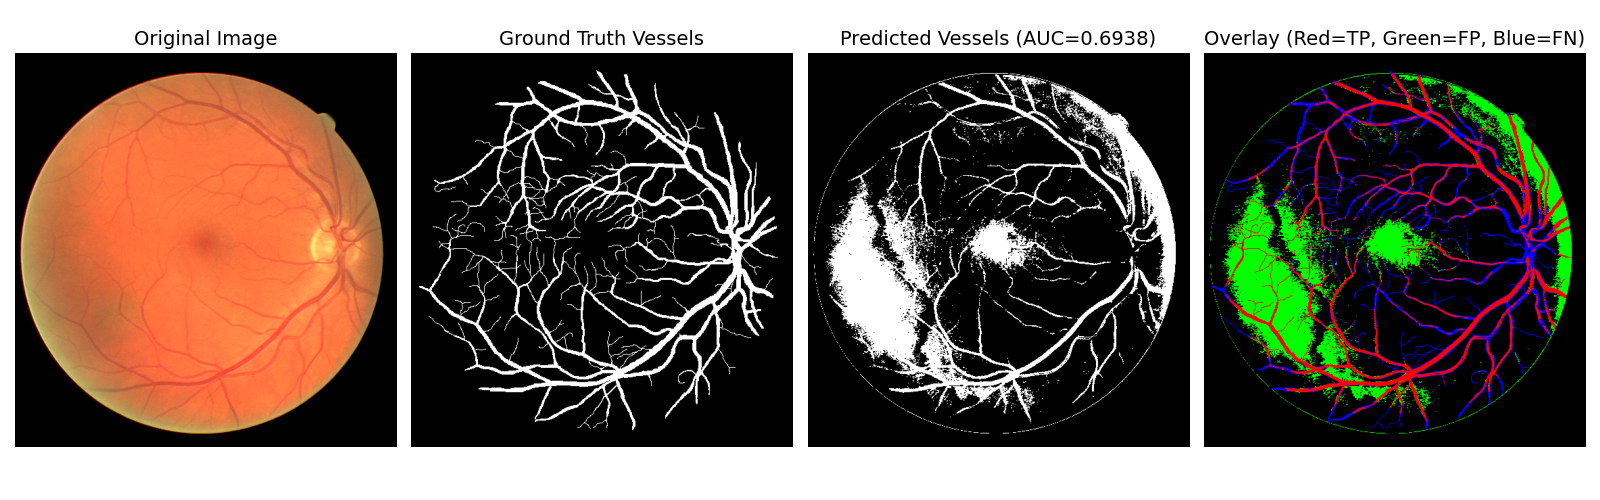
\includegraphics[scale=0.35]{Figures/3 Optimized 1st.png}
        \vspace{-0.5cm}
        \caption{First Best Example (AUC=0.6938)}
        \label{fig:opt1}
    \end{subfigure}
    \begin{subfigure}[H]{\textwidth}
        \centering
        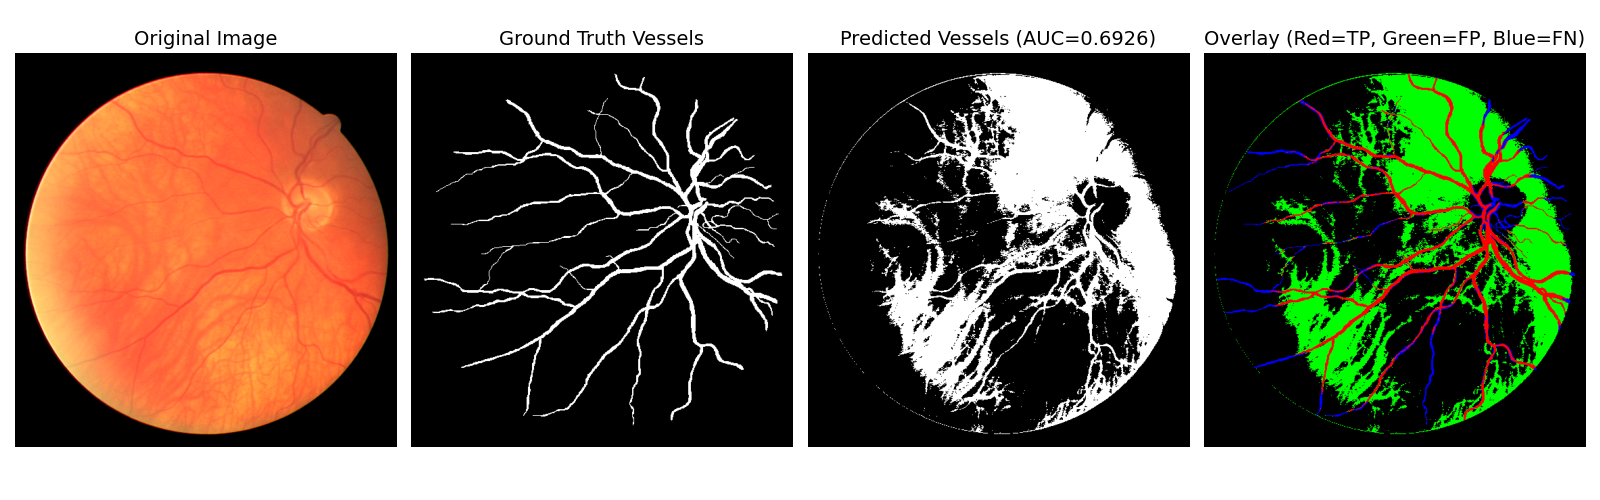
\includegraphics[scale=0.35]{Figures/3 Optimized 2nd.png}
        \vspace{-0.5cm}
        \caption{Second Best Example (AUC=0.6926)}
        \label{fig:opt2}
    \end{subfigure}
    \begin{subfigure}[H]{\textwidth}
        \centering
        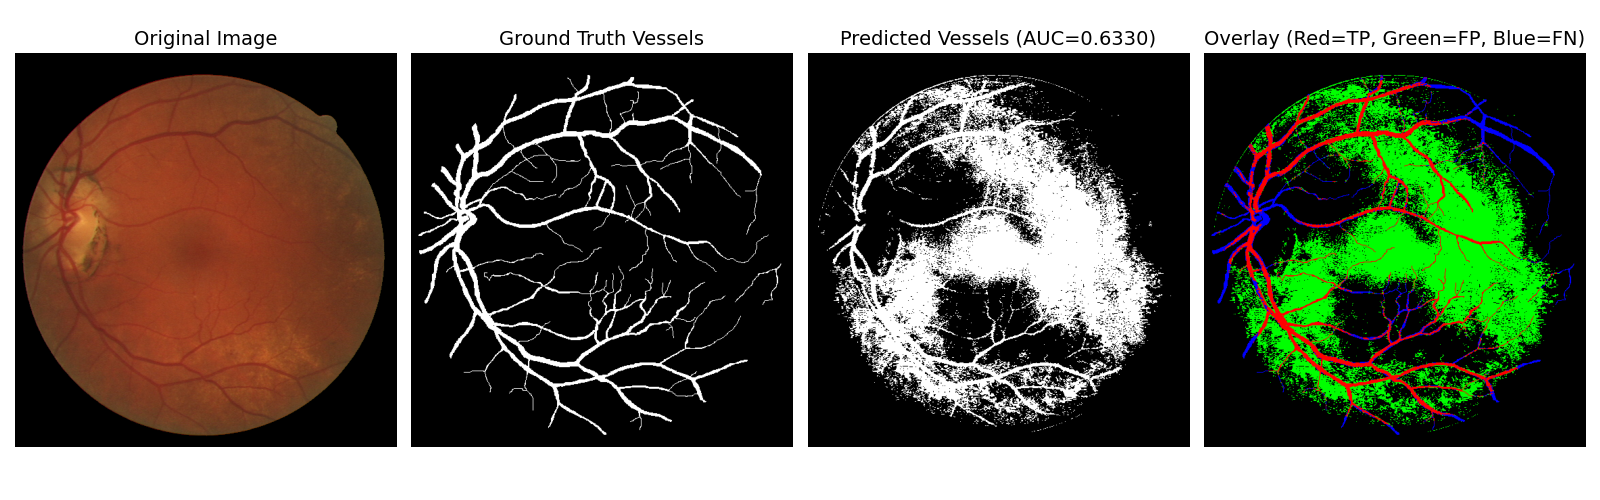
\includegraphics[scale=0.35]{Figures/3 Optimized 3rd.png}
        \vspace{-0.5cm}
        \caption{Third Best Example (AUC=0.6330)}
        \label{fig:opt3}
    \end{subfigure}
    \caption{Optimized K-means: Top 3 Examples}
    \label{fig:opt}
\end{figure}
\noindent
As we can see, the biggest problem is that there are a lot of false positive pixels (FP, Green) in the segmentation results, which means that their colors are difficult to distinguish from blood vessels. \\
Therefore, we apply \textbf{image augmentation} to enhance the color differences, which may help to improve the segmentation performance. 
\subsubsection{Image Augmentation with Optimized K-means}
Image augmentation was further applied to enhance the quality of vessel segmentation. By pre-enhancing the input images, the clustering algorithm produces improved segmentation results. The results corresponding to the 3 best examples above after applying image augmentation are shown in Figure~\ref{fig:opt_aug} below. 
\begin{figure}[H]
    \centering
    \begin{subfigure}[H]{\textwidth}
        \centering
        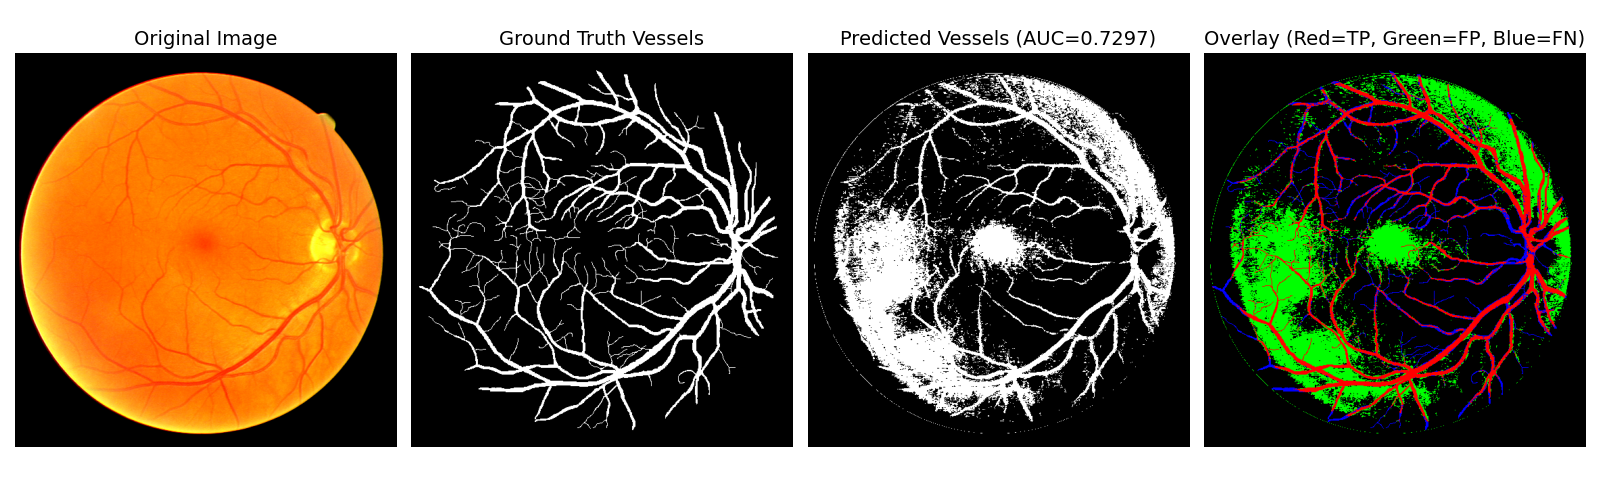
\includegraphics[scale=0.35]{Figures/4 Optimized 1st.png}
        \vspace{-0.5cm}
        \caption{First Best Example (AUC=0.6938 $\rightarrow$ \textcolor{red}{0.7297})}
        \label{fig:opt_aug1}
    \end{subfigure}
    \begin{subfigure}[H]{\textwidth}
        \centering
        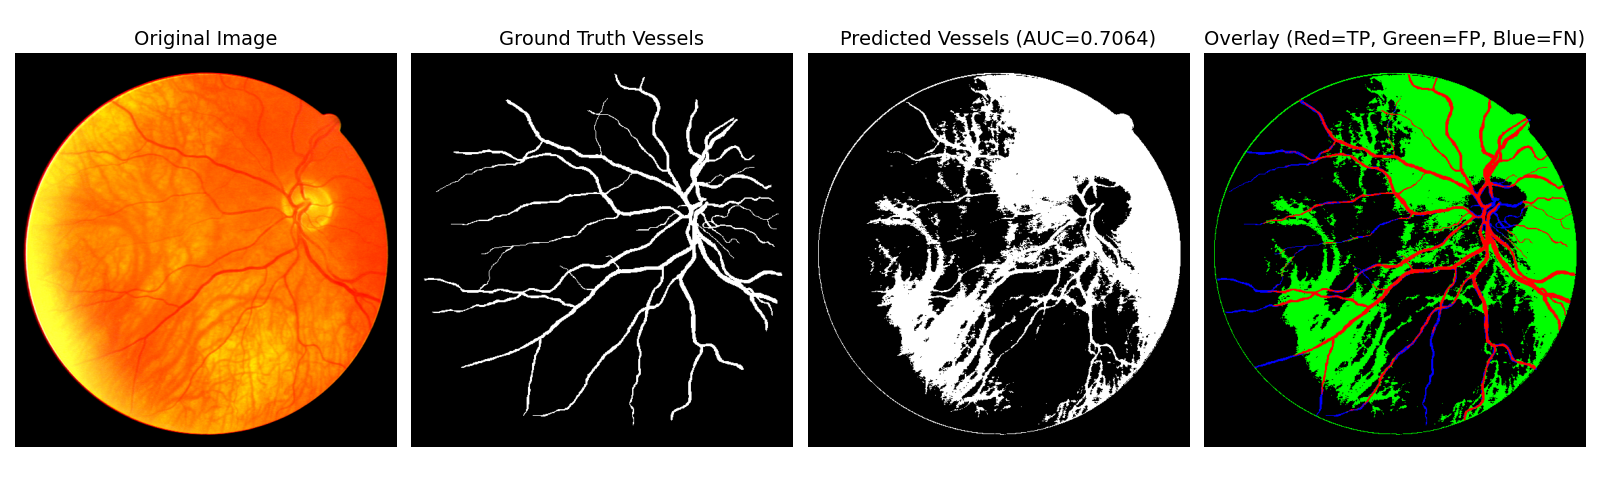
\includegraphics[scale=0.35]{Figures/4 Optimized 2nd.png}
        \vspace{-0.5cm}
        \caption{Second Best Example (AUC=0.6926 $\rightarrow$ \textcolor{red}{0.7064})}
        \label{fig:opt_aug2}
    \end{subfigure}
    \begin{subfigure}[H]{\textwidth}
        \centering
        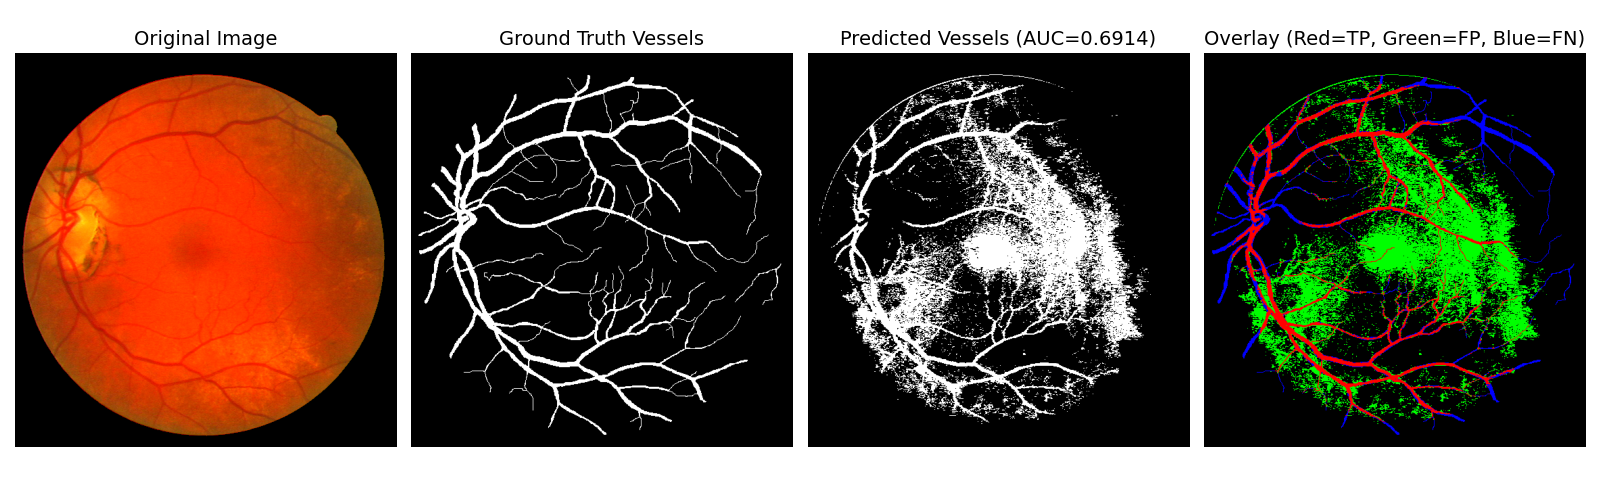
\includegraphics[scale=0.35]{Figures/4 Optimized 3rd.png}
        \vspace{-0.5cm}
        \caption{Third Best Example (AUC=0.6330 $\rightarrow$ \textcolor{red}{0.6914})}
        \label{fig:opt_aug3}
    \end{subfigure}
    \caption{Optimized K-means with Augmentation: Corresponding 3 Examples}
    \label{fig:opt_aug}
\end{figure}
\noindent
Apparently, the results are much better now. The false positive pixels (FP, Green) are significantly reduced, and the segmentation results are more accurate. 
\subsubsection{Direction-enhanced K-means Clustering}
In order to further improve segmentation, we try to take advantage of the fact that blood vessels are long and thin. So we incorporate the \textbf{gradient-based features} into the clustering process. \\
In this approach, the original RGB features are augmented with gradient magnitude and gradient direction (obtained via the Sobel filter), forming an enhanced feature vector. Such directional information helps to better delineate vessel boundaries. Two merging strategies (merging the top 3 and top 5 vessel clusters) were tested, as illustrated in the following figures (Figure~\ref{fig:de}).
\begin{figure}[H]
    \centering
    \begin{subfigure}[H]{\textwidth}
        \centering
        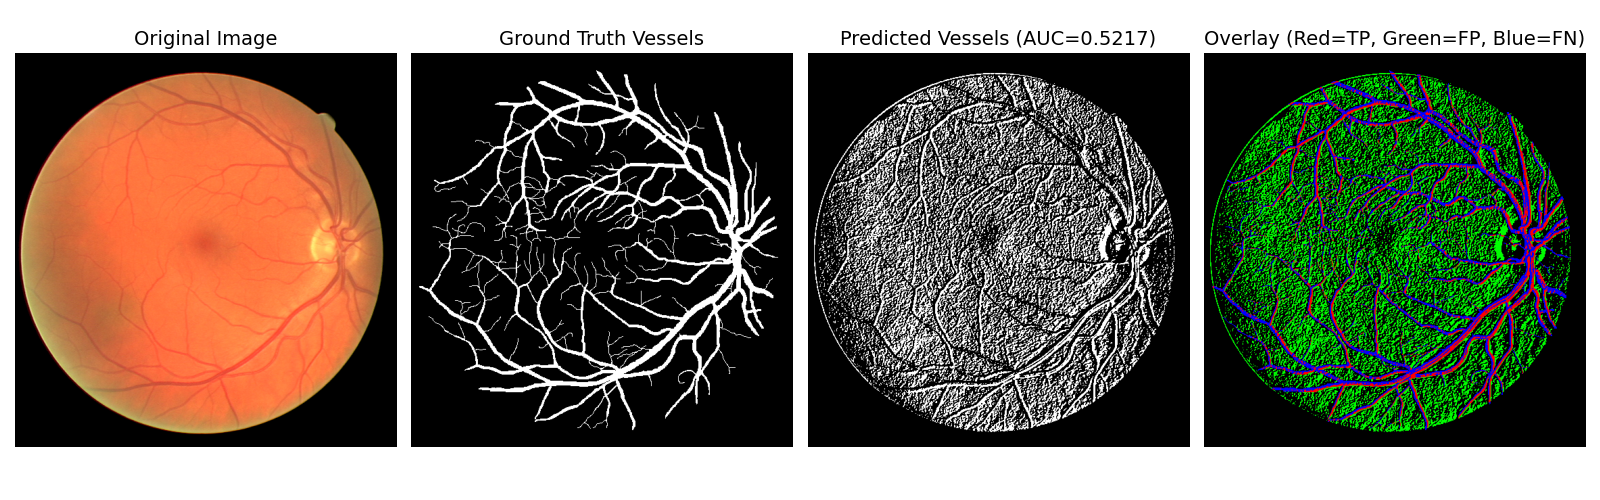
\includegraphics[scale=0.35]{Figures/5 Directed (Merge 3 Clusters).png}
        \vspace{-0.5cm}
        \caption{Merging Top 3 Clusters (AUC=0.5217)}
        \label{fig:de3}
    \end{subfigure}
    \begin{subfigure}[H]{\textwidth}
        \centering
        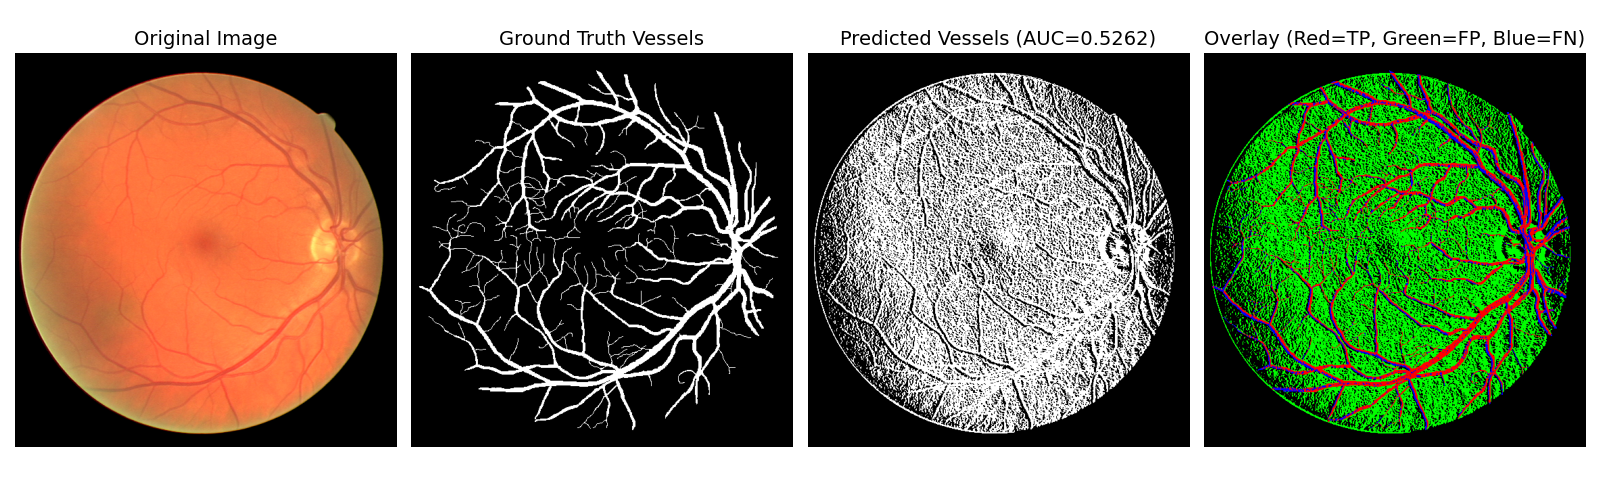
\includegraphics[scale=0.35]{Figures/5 Directed (Merge 5 Clusters).png}
        \vspace{-0.5cm}
        \caption{Merging Top 5 Clusters (AUC=0.5262)}
        \label{fig:de5}
    \end{subfigure}
    \caption{Direction-enhanced K-means}
    \label{fig:de}
\end{figure}
\noindent
We can see that when the number of merged clusters increases, the true positive pixels (TP, Red) and false positive pixels (FP, Green) increase simultaneously. This is because the more top clusters we merge, the more TP and FP pixels are included in the final segmentation mask. \\ 
After applying image augmentation, additional improvements can be observed (see Figure~\ref{fig:de_aug}).
\begin{figure}[H]
    \centering
    \begin{subfigure}[H]{\textwidth}
        \centering
        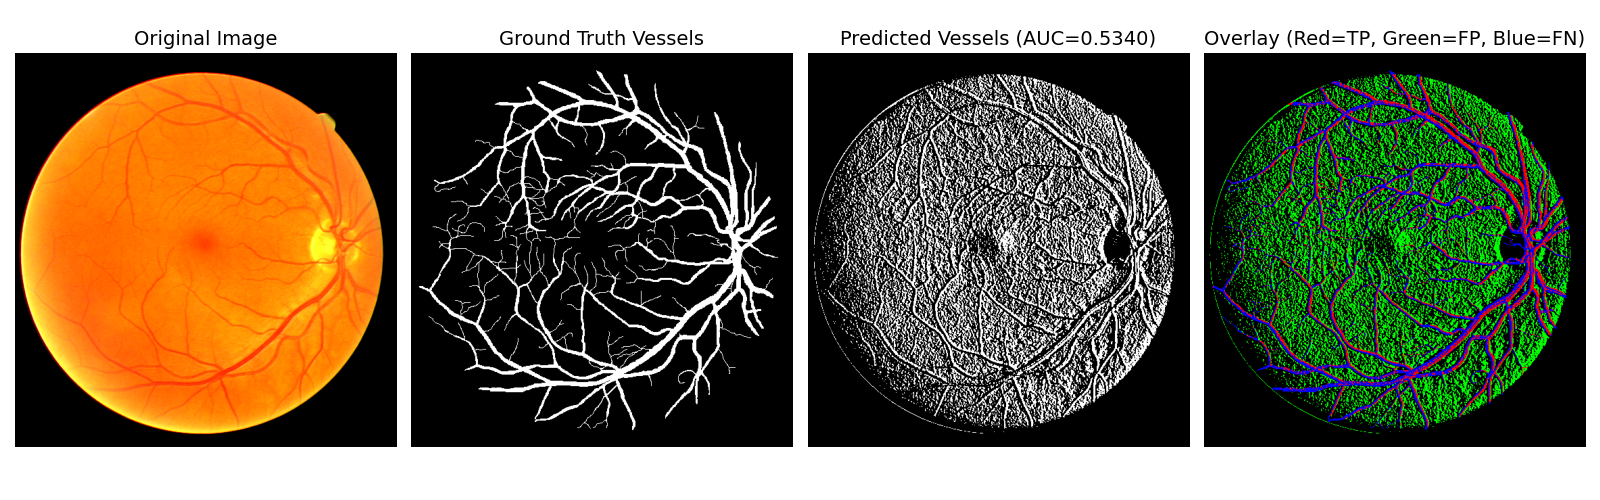
\includegraphics[scale=0.35]{Figures/6 Directed (Merge 3 Clusters).png}
        \vspace{-0.5cm}
        \caption{Merging Top 3 Clusters (AUC=0.5217 $\rightarrow$ \textcolor{red}{0.5340})}
        \label{fig:de_aug3}
    \end{subfigure}
    \begin{subfigure}[H]{\textwidth}
        \centering
        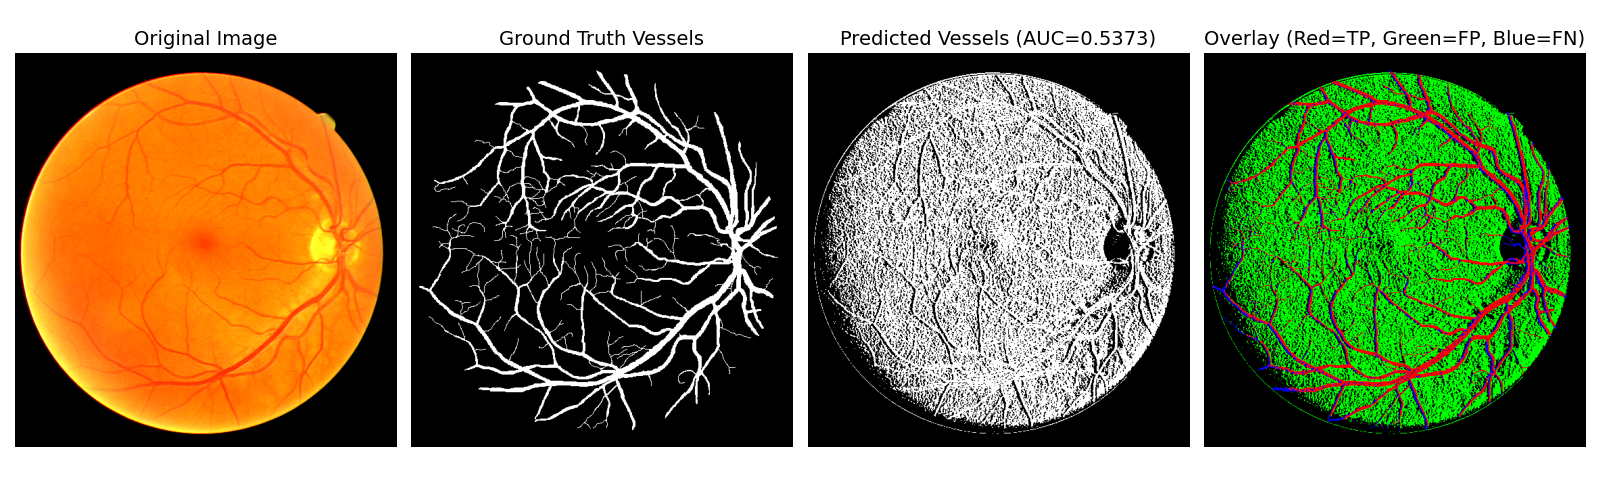
\includegraphics[scale=0.35]{Figures/6 Directed (Merge 5 Clusters).png}
        \vspace{-0.5cm}
        \caption{Merging Top 5 Clusters (AUC=0.5262 $\rightarrow$ \textcolor{red}{0.5373})}
        \label{fig:de_aug5}
    \end{subfigure}
    \caption{Direction-enhanced K-means with Augmentation}
    \label{fig:de_aug}
\end{figure}
\noindent
The overall performance of the direction-enhanced K-means is not as good as previous methods, but it still provides a different perspective on the segmentation task by showing the potential of incorporating gradient features. Also, the results are shown in a different style, which is quite interesting. \\
Besides, we can also see the small improvement of the AUC value after applying image augmentation, which further verify the effectiveness of this technique. 
\subsubsection{Performance Evaluation and Comparison}
The performance of the segmentation approaches is evaluated using accuracy, sensitivity, specificity, F1-score, and AUC value, which refer to related studies. \\
Table~\ref{tab:performance} summarizes the performance comparison between the classic K-means and the optimized K-means methods, both before and after applying image augmentation. (Not include the direction-enhanced K-means is because it is just a try and not the main focus of this project.) 
\begin{table}[H]
    \centering
    \caption{Performance Comparison: Before (Black) and After (Red) Image Augmentation}
    \label{tab:performance}
    \begin{tabular}{lcc}
    \hline
    \textbf{Metric} & \textbf{Classic K-means} & \textbf{Optimized K-means} \\
    \hline
    Accuracy & $0.8062 \rightarrow \textcolor{red}{0.8404}$ & $0.6193 \rightarrow \textcolor{red}{0.6938}$ \\
    Sensitivity & $0.2228 \rightarrow \textcolor{red}{0.2805}$ & $0.5862 \rightarrow \textcolor{red}{0.6138}$ \\
    Specificity & $0.8898 \rightarrow \textcolor{red}{0.9200}$ & $0.6247 \rightarrow \textcolor{red}{0.7057}$ \\
    F1 Score   & $0.2270 \rightarrow \textcolor{red}{0.3115}$ & $0.2802 \rightarrow \textcolor{red}{0.3393}$ \\
    AUC value    & $0.5563 \rightarrow \textcolor{red}{0.6003}$ & $0.6054 \rightarrow \textcolor{red}{0.6598}$ \\
    \hline
    \end{tabular}
\end{table}
\noindent
Through comparison of evaluation metrics, it is evident that image augmentation has a positive impact on both K-means algorithms. \\
Although classic K-means shows better performance in accuracy and specificity, the optimized K-means algorithm demonstrates significant advantages in key metrics such as sensitivity and AUC value, especially when combined with image augmentation techniques, providing more effective discrimination between vessel and non-vessel regions. \\
This suggests that the optimized K-means algorithm has stronger recognition capabilities in vessel segmentation applications, making it particularly suitable for medical image analysis tasks that require higher detection rates.
\subsubsection{Conclusion and Future Work}
For this part, we explored classical unsupervised machine learning techniques for retinal vessel segmentation. Through the use of K-means clustering and its optimized variations, including image augmentation and the incorporation of gradient features, the proposed methods demonstrated significant improvements in segmentation performance as measured by standard evaluation metrics. \\
For future work, the following directions are suggested:
\begin{itemize}
    \item \textbf{Improved Image Augmentation:} In addition to traditional geometric transformations (e.g., rotation and flipping), consider advanced photometric adjustments, including saturation, hue, and white balance to mimic different lighting conditions. 
    \item \textbf{Enhanced Feature Extraction:} Incorporating additional features beyond raw RGB values and gradients, such as texture descriptors, fractal-based features, or deep feature representations, to better capture vessel morphology.
\end{itemize}


\subsection{Random Forest Classification}
The random forest algorithm, a robust ensemble learning method, can be effectively applied to retinal image segmentation by leveraging its ability to classify pixels into anatomical or pathological regions through supervised learning. In this context, features such as pixel intensity, texture gradients, local binary patterns, and responses to edge-detection filters (e.g., Sobel or Gabor) are extracted from retinal images to capture structural details of blood vessels, lesions, or the optic disc. During training, the algorithm constructs multiple decision trees, each trained on random subsets of the data and features, to predict pixel-wise labels from annotated ground-truth masks. At inference, the ensemble aggregates predictions across trees, assigning each pixel to the most probable class (e.g., vessel vs. non-vessel), while mitigating overfitting through majority voting. 

\subsubsection{Training Process}
The gist of Random Forest is to build multiple decision trees and aggregate their predictions. The training process involves the following steps:
\begin{enumerate}
    \item \textbf{Feature Extraction}: Extract features from the training images, in our cases, the features are simply the RGB values of the pixels.
    \item \textbf{Random Sampling}: Randomly select subsets of the training data and features to build each decision tree, ensuring diversity among trees.
    \item \textbf{Tree Construction}: For each subset, construct a decision tree by recursively splitting the data based on feature thresholds that maximize information gain or minimize Gini impurity (which is the taken approach).
    
\textbf{Gini impurity} (for class \( k \)):  
\[
G = 1 - \sum_{k=1}^K p_k^2
\]  
where \( p_k \) is the proportion of samples of class \( k \) in the node.  

\textbf{Information gain} (using entropy \( H \)):  
\[
H = -\sum_{k=1}^K p_k \log p_k
\]  
\[
\text{Information Gain} = H_{\text{parent}} - \sum_{\text{child}} \frac{N_{\text{child}}}{N_{\text{parent}}} H_{\text{child}}
\]  

    \item \textbf{Prediction Aggregation}: At inference, aggregate predictions from all trees using majority voting to assign the final class label to each pixel.
\end{enumerate}

    Through the whole training process, totally 10 images, \(10 \times 584 \times 565 = 3299600\) pixels are trained upon. The pixels are separeted into 3 classes: 0 for masked boundary, 1 for background and 2 for blood vessels. Below is a typical prediction result given by the classifier:

    \begin{figure}[H]
        \centering
            \centering
            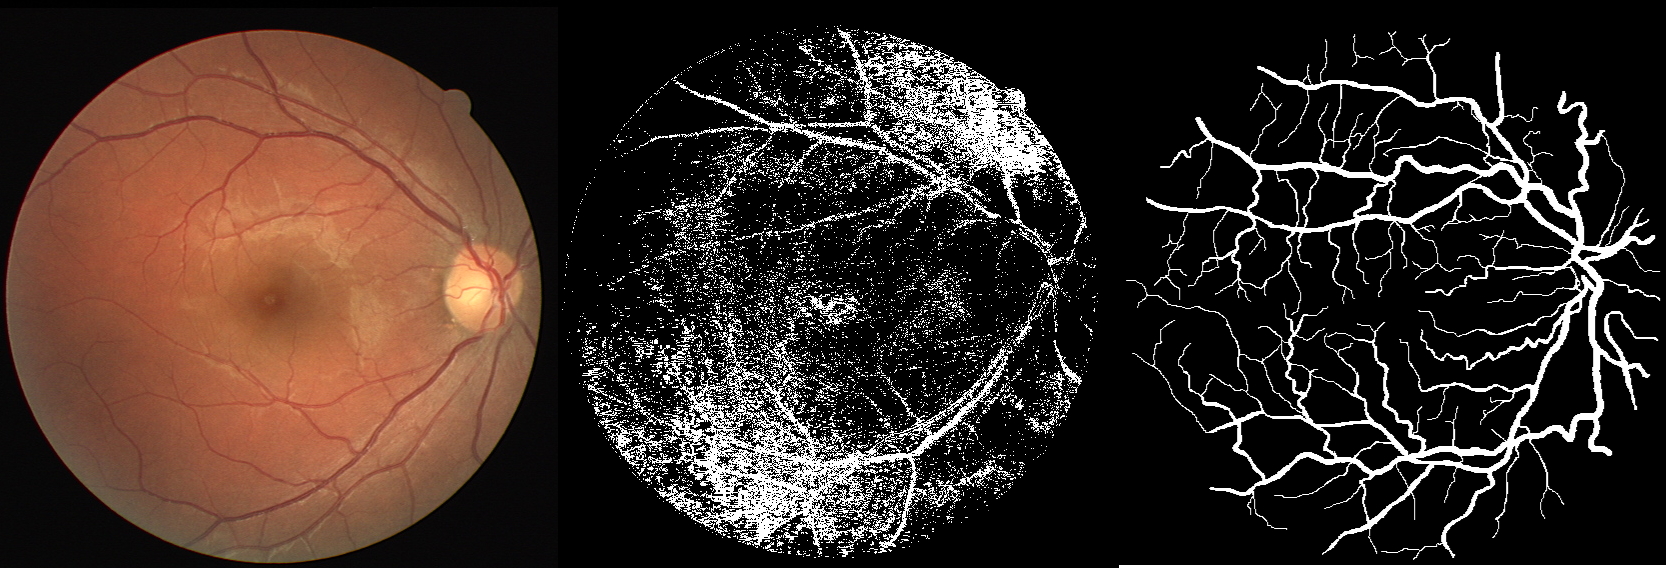
\includegraphics[scale=0.4]{Figures/mjc.png}
            \caption{1st image is the original image, 2nd image is the manually labeled image for training, 3rd image is the predicted image by the random forest algorithm.}\label{fig:mjct27}
    \end{figure}
    \noindent

    \begin{table}[H]
        \caption{Metrics for the segmentation Task}
        \begin{tabular}{ccccc}
                         & precision & recall & f1-score & support \\
        background       & 0.91      & 0.80   & 0.85     & 198755  \\
        retinal          & 0.24      & 0.44   & 0.31     & 29073   \\
        accuracy         &           &        & 0.75     & 227828  \\
        weighted average & 0.82      & 0.75   & 0.78     & 227828  
        \end{tabular}
    \end{table}




\subsection{Conclusion}



\subsubsection{Reflection and Future Work}
Despite our efforts, the output given by our classifier are still far from satisfactory compared with the the provided manual data used for training. We want to identify some potential reasons and improvement that can be made:
\begin{itemize}
    \item \textbf{The limiation of RGB under different Saturation}: Both training and testing images are of different saturation, meaning that the pixels of same RGB value may be in completely different category in different images. This suggests that using only RGB value for classification is vastly insufficient. We can try to use other features such as texture, gradient, etc. to improve the performance. Further more, to make sure localness between pixels is reflected in training, we can consider including the pixel's neighbors's color in the feature set.

    \item \textbf{Feature Selection}: 
    
    \item \textbf{Hyperparameter Tuning}: 
\end{itemize}

\end{document}
